

\chapter{Elektronik}
\label{chap:elektronik}
\section{Das Gehirn des Bootes}
Für die Steuerung des Bootes wird ein Raspberry Pi Zero W 1.1 verwendet. Dieser verfügt über ausreichend Rechenleistung, um alle notwendigen Berechnungen in Echtzeit durchzuführen. Er verfügt über einen einkernigen ARM Prozessor, der mit 400 MHz getaktet ist. Sein Arbeitsspeicher beträgt 512 Megabyte. Er ist 6,5 mal 3,2 cm gross und wiegt nur 9 Gramm.

Auf dem Raspberry Pi läuft ein Debian basiertes GNU/ Linux Betriebssystem. Im Kapitel Autonomie wird auf die Software detailliert eingegangen. 
Der Raspberry Pi Zero W 1.1 kann über WLAN nach den Spezifikationen 802.11 b/g/n sowie über Bluetooth 4.1 und Bluetooth Low Energy (BLE) kommunizieren. Die WLAN Verbindung wird benutzt, um mit dem autonomen Segelboot zu kommunizieren. Über die Verbindung kann der Rechner drahtlos aufgesetzt und eingerichtet werden. Auch die Übermittlung von Zielkoordinaten erfolgt über diese Verbindung. Die Bluetoothverbindung wird nicht benutzt.
\begin{figure}
    \centering
    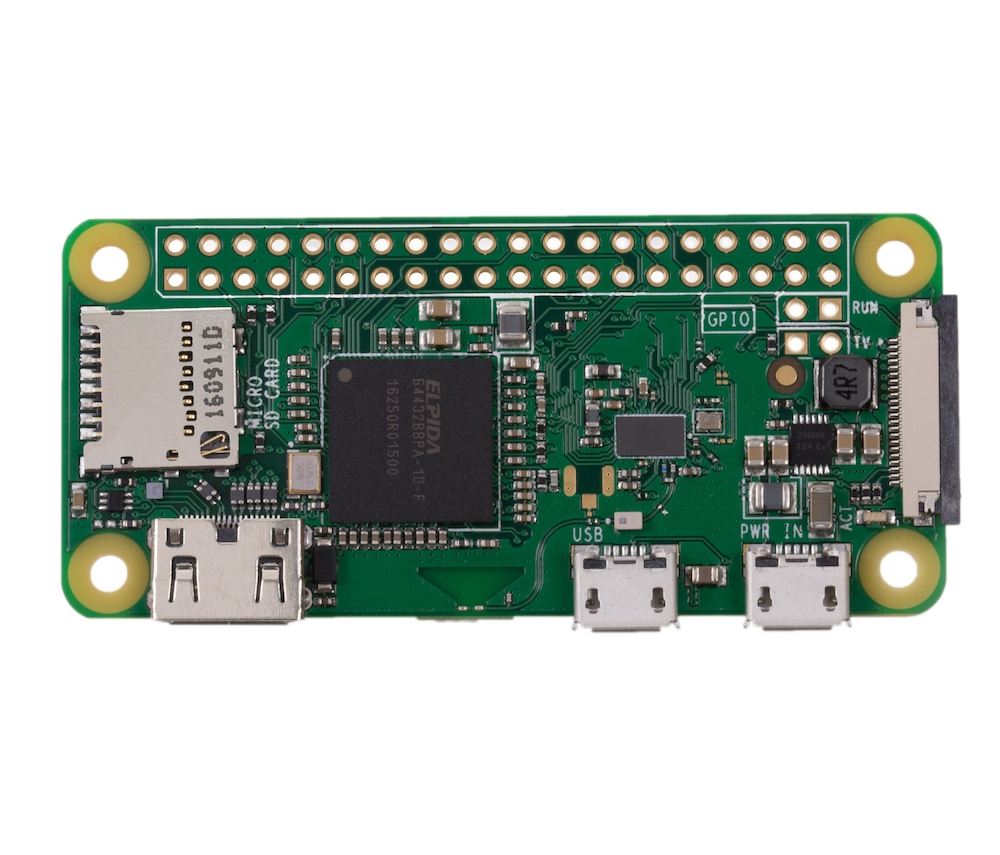
\includegraphics[width=0.5\linewidth]{assets/raspi Zero.jpg}
    \caption{Raspberry Pi Zero }
    \label{fig:enter-label}
\end{figure}

Die in den unmittelbar nachfolgenden Abschnitten beschriebenen Sensoren und Aktuatoren sowie die Energieversorgung werden über die 40 GPIO (general-purpose input/output) Pins angeschlossen. 

Der Raspberry Pi Zero W 1.1 wird mit 5 V Gleichspannung betrieben. Sein Stromverbrauch ist sehr bescheiden. Seine maximale Stromaufnahme liegt bei 1,2 A.
\cite{noauthor_raspberry_2023} im Leerlauf braucht er aber nur 120 mA.
\cite{noauthor_stromverbrauch_nodate}
\section{Sensoren und Aktuatoren}
\subsection{Positionsestimmung (GPS)}
Zur Positionsbestimmung, also der Bestimmung des aktuellen Standorts des Segelboots, werden Funksignale des bekannten US-amerikanischen satellitenbasierten Global Positioning Systems (GPS) (deutsch Globales Positionsbestimmungssystem) offiziell NAVSTAR GPS verwendet. Dafür wird das Empfängermodul Whadda Neo 7M der belgischen Velleman Group nv verwendet, welches alternativ Signale des entsprechenden russischen Systems GLONASS empfangen kann.
\begin{figure}[H] 
    \centering
    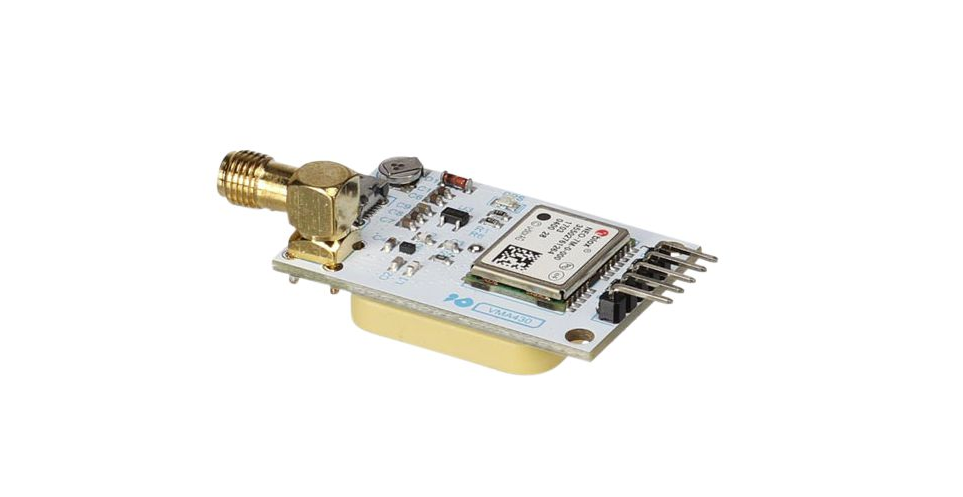
\includegraphics[width=1\linewidth]{gps.png}
    \caption{GPS Modul}
    \label{fig:gps}
\end{figure}
Das Modul verfügt über eine Micro-USB Schnittstelle. Diese wird aber nicht verwendet, weil der Raspberry Pi Zero W 1.1 zwar über zwei Micro-USB verfügt, die nicht benutzt werden, Kabel mit zwei männlichen Micro-USB Steckern aber nicht existieren und in den USB Standards nicht vorgesehen sind. \\ \\
Das Modul wird über die eben falls vorhandenen Pins mit dem Raspberry Pi Zero W 1.1 verdrahtet und  kommuniziert über eine serielle Verbindung. Die Pins 2 (TX) und 3 (RX) werden dabei mit den Pins 10 und 8 des Raspberry Pi Zero W 1.1 verbunden. Das Modul wird mit 5 V betrieben. Dazu wird sein Pins 5 (VCC) mit der 5 V Gleichspannungsleitung und sein Pin 4 (GND) mit der Ground Leitung der Stromversorgung verbunden.   
\begin{figure}[H]
    \centering
    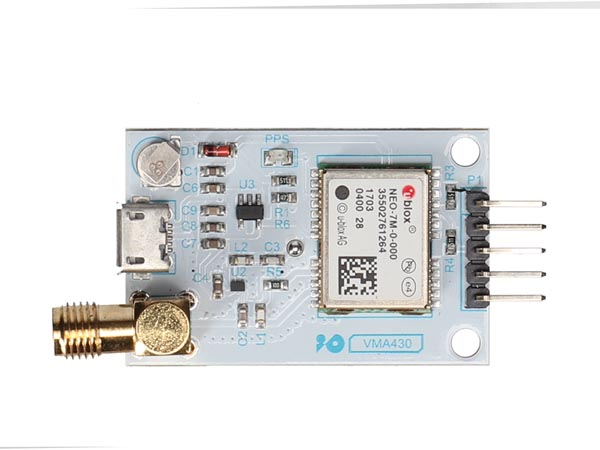
\includegraphics[width=0.75\linewidth]{vma430_front-1.jpg}
    \caption{GPS Modul - Oberseite}
    \label{fig:enter-label}
\end{figure}
Das Modul wird unter Deck im Rumpf des Bootes platziert. Weil für die Deckplatte eine dünne Sperrholzplatte verwendet wird, kann auf eine externen Empfangsantenne verzichtet werden. Die vorhandene SMA Antennen Steckbuchse bleibt damit unbenutzt. Es wird die eingebaute keramische Patchantenne verwendet. In der unmittelbar unten stehenden Abbildung ist diese als rosa Fläche mit einem metallenen Knopf auf einem beigen Körper sichtbar.
\begin{figure}[H]
    \centering
    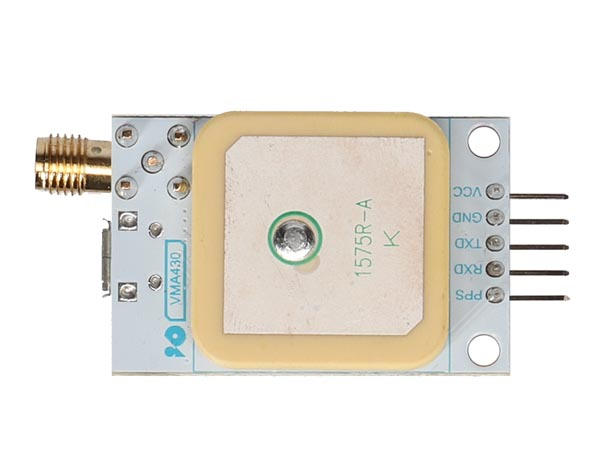
\includegraphics[width=0.5\linewidth]{vma430_back-1.jpg}
    \caption{GPS Modul - Unterseite}
    \label{fig:enter-label}
\end{figure}

\subsection{Gyro und Magnetometer}

Zur Bestimmung der Richtung des Segelboots dient ein Magnetometer. Ein Magnetometer ist eine sensorische Einrichtung zur Messung magnetischer Flussdichten \cite{noauthor_magnetometer_2023}. Im vorliegenden Projekt wird das Magnetometer dafür eingesetzt, um damit einen Magnetkompass zu realisieren, indem das erdmagnetische Feld dreidimensional erfasst wird, um daraus die Bootsrichtung abzuleiten. Dieses Verfahren wird auch in Smartphones zur Richtungsbestimmung angewendet.

Im vorliegenden Projekt wird dafür das Sensormodul Purecrea GY-273 QMC5883L der deutschen Purecrea GmbH vorgesehen. Das Modul ist zusätzlich mit einem Gyroskop (Deutsch: Kreiselinstrument) ausgestattet. Auch damit kann die Bewegung des Segelboots erfasst werden. Ausserdem erlaubt es die Bestimmung der Schräglage des Segelbootes. Im vorliegenden Projekt wird dieser Wert aber nicht erfasst und ausgewertet

\begin{figure}[H]
    \centering
    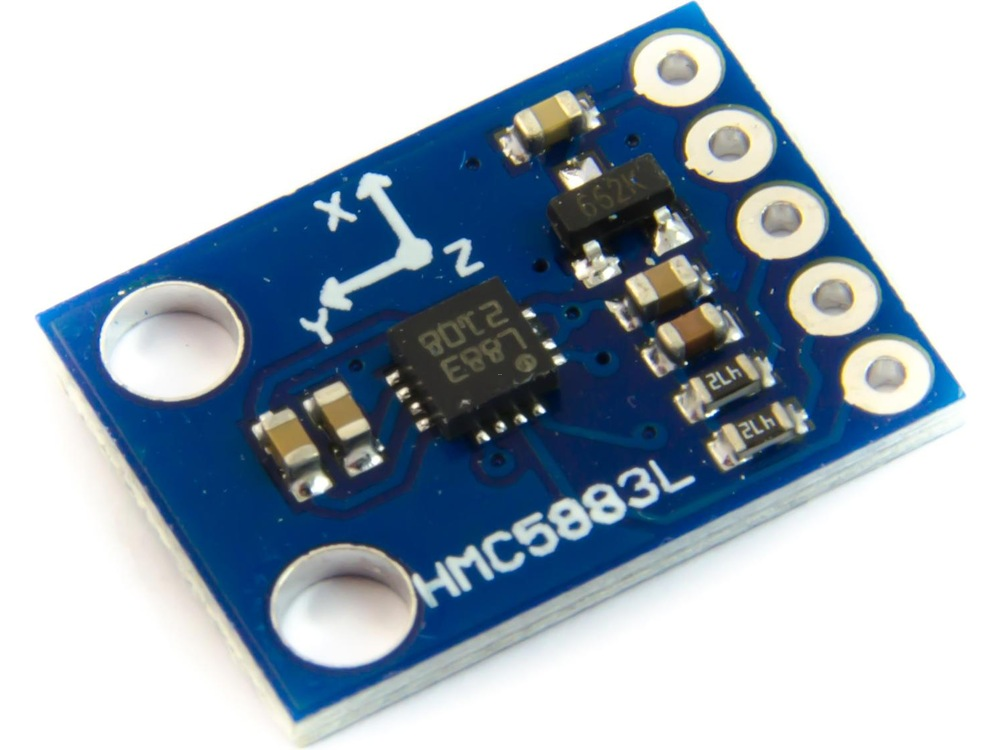
\includegraphics[width=0.5\linewidth]{assets/magnetometer.jpg}
    \caption{Gyro und Magnetometer}
\end{figure}

Das Sensormodul wird mit einer Eingangsspannung von 3-5 V Gleichspannung betrieben. Pin 1 (GND) wird dafür mit der Ground Leitung und sein Pin 2 (VCC) wird mit der der 5 V Gleichspannungsleitung der Stromversorgung verbunden.

Die Kommunikation mit dem Raspberry Pi Zero W 1.1 erfolgt über eine serielle Verbindung. Der Pin 4 (SCL) und der Pin 5 (SDA) des Moduls werden dafür mit den Pins 5 und 19 des Raspberry Pi Zero W 1.1 verdrahtet.

\subsection{Eigenentwicklung des Windrichtungssensor}
Der Windrichtungssenor muss selbst entwickelt und gebaut werden, da die am Markt angebotenen Windrichtungsmesser entweder zu gross und zu schwer sind, Energiemengen benötigen, die auf dem autonomen Segelboot nicht zur Verfügung stehen oder unerschwinglich teuer sind.

Windrichtungssensoren lassen sich in zwei unterschiedliche Typen einteilen. Der erste Typ verwendet ein Potenziometer zur Richtungsbestimmung. Solche Messgeräte sind mechanisch sehr leicht umzusetzen, da dazu lediglich ein kleiner Flügel an der Achse eines Potenziometers befestigt werden muss. Die Position des Flügels kann damit über einen analogen Input Pin mit einem Mikrocontroller eingelesen und daraus die Richtung des Windes abgeleitete werden. Der Nachteil dieses Typs ist, dass die freie Drehung der Achse durch die Reibung das Potenziometers stark abgebremst wird. Dieser Typ wird daher nicht weiter verfolgt.

Der andere Type verwendet Hallsensoren, welche den Hall-Effekt zur Messung von 
Magnetfeldern nutzen \cite{noauthor_hall-sensor_2023}. Sie sind passive Sensoren, die den Spannungsunterschied messen, der an einem elektrischen Leiter erzeugt wird, wenn ein Magnetfeld senkrecht zur Fliessrichtung eines elektrischen Stroms steht \cite{noauthor_alles_nodate}. Um die Rotation eines Objektes mittels Hallsensoren zu messen, gibt es die folgenden zwei Möglichkeiten.

Bei der ersten Variante wird um ein abwechselnd magnetisch positiv und magnetisch negativ geladenes rundes Objekt mehrere Hallsensoren platziert. Damit kann dann die Drehung des Objektes gemessen werden. Diese Variante ist praktisch schwierig umzusetzen, weil viele Hall Sensoren präzis kreisförmig um eine Achse angeordnet werden müssen. Dafür müssten die Hallsensoren in enger Folge auf einer individuell entworfenen Platine verlötet werden. Der Entwurf einer solchen Platine ist anspruchsvoll, mit deren Herstellung müssten Auftragsfertiger beauftragt werden, was hohe Kosten verursachen würde. Weil die Hallsensoren sehr eng aneinander platziert werden müssten, müssten sogenannte SMD Varianten (Surface Mountable Device; deutsch: oberflächenmontierbare Bauteile) verwendet werden, die ohne Bohrungen direkt auf die Oberfläche der Platine gelötet werden. Es braucht dafür eine spezielle Löttechnik und die Gefahr, dass Bauteile beim Lötvorgang den Hitzetod sterben, ist erheblich, wenn der Lötende über wenig Übung verfügt. Diese Varianten wird daher nicht weiter verfolgt.

Die zweite Varianten ist praktisch einfacher umzusetzen. Statt normale Hall Sensoren werden dabei spezielle, sogenannten Rotary Hall (deutsch rotierende magnetische Hall) Encoder verwendet. Ein Encoder (oder Messwertgeber) dient in der Antriebstechnik zur Signalbildung aus mechanischen Bewegungen. Er erkennt die Position einer Antriebseinheit (Welle) und gibt diese als elektrisches Signal aus.\cite{noauthor_was_nodate} Rotary Hall Encoder sind komplexe Bauteile, die fast immer als System-on-Chip gefertigt, in dem integrierte Hall-Elemente, analoges Frontend und digitale Signalverarbeitung in einem einzigen Gerät integriert sind. Zur Messung des Winkels wird nur ein einfacher zweipoliger Magnet benötigt, der sich der sich über oder unter der Mitte des Chips dreht.

Zur Funktionsweise von Rotary Hall Encodern: Josef Janisch, Understanding Integrated Hall Effect Rotary Encoders, Nov 1, 2006 1:00am, auf Fierce Electonics \cite{janisch_understanding_2006}.

Für das vorliegende Projekt wird ein Windsensor auf der Basis eines Rotary-Hall-Encoders vorgezogen. Dabei wird der auf einem Adapterboad gelötete AS5040-ASST der österreichischen ams-OSRAM AG verwendet. Das ist ein berührungsloser Rotary Hall Encoder für genaue Winkelmessung über eine volle Umdrehung von 360$^\circ$.  Die absolute Winkelmessung liefert eine sofortige Anzeige der die Winkelposition des Magneten mit einer Auflösung von 0,35$^\circ$ = 1024 Positionen pro Umdrehung. Diese digitalen Daten sind als serieller Bitstrom und als PWM (Pulsweitenmodulation) Signal zur Verfügung. Für das vorliegende Projekt wird nur der serielle Bitstrom verwendet. Der Pin A des Adapterboards wird dabei mit dem BMC23 Pin des Raspberry Pi Zero W 1.1 und der Pin B des Adapterboards mit dem BMC24 Pin des Raspberry Pi Zero W 1.1 verbunden.

Der Encoder kann mit 3,3V oder 5V betrieben werden. Quellen für beide Spannungen sind auf dem Segelboot vorhanden. Es wird ein 3.3V Pin des Raspberry Pi Zero W 1.1 genutzt.

\begin{figure}
    \centering
    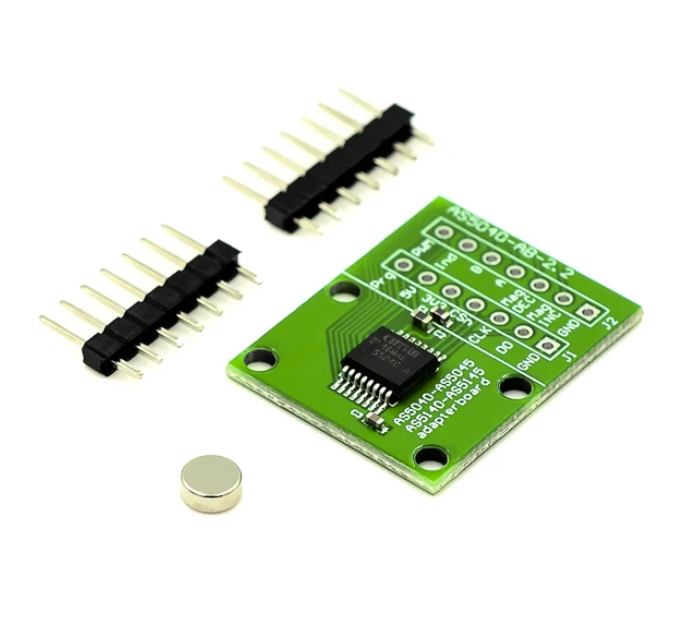
\includegraphics[width=0.5\linewidth]{assets/as5040image.png}
    \caption{AS5040-ASST mit Adapter Board}
    \label{fig:as5040}
\end{figure}

Entwurf und Bau de Windrichtungssensors aus 3D gedruckten Teilen. 
Die restlichen Teile des Windrichtungssensors werden von Grund auf selbst entworfen und gebaut. Es handelt sich dabei um die Bodenplatte, das Gehäuse, die Welle und den Windflügel. Die vier Teile wurden mit dem CAD Programm entworfen und mit dem 3D Drucker gedruckt.

Der drehbare Windflügel verfügt am Ende über ein Segel, damit er sich selbständig in den Wind dreht. Er ist 15 cm lang.
\begin{figure}[H]
    \centering
    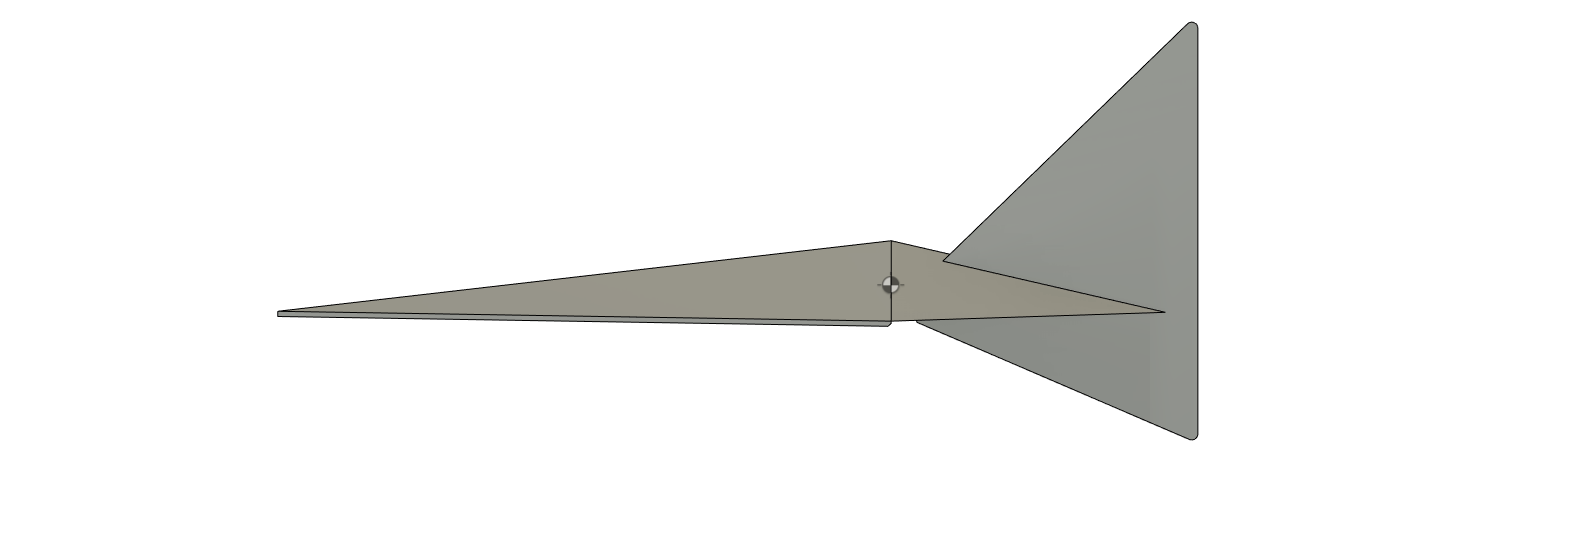
\includegraphics[width=0.75\linewidth]{assets/windsensor_top.png}
    \caption{Windflügel}
    
\end{figure}

Der Windflügel wird fest mit der Welle verbunden. Diese wird dann von oben ins leere Gehäuse geführt. Das Gehäuse weist dafür eine Öffnung auf, in welcher ein Kugellager verleimt wird, damit sich die Welle frei drehen kann. Die Konstruktion ist so ausgelegt, dass der Massemittelpunkt unabhängig von der Lage des Segelboots genau auf dem Drehpunkt des Windflügels liegt. Damit ist sichergestellt, dass auch bei den häufigen Schräglagen korrekte Werte ermittelt werden.

Das Gehäuse steht auf einer am Deck des Segelbootes gefestigten Grundplatte. Es hebt den Windflügel in den Wind und schützt die Adapterplatte mit dem Rotary-Hall-Encoder vor der Witterung und Wellen.

Die Grundplatte weist auf der Gehäuseseite eine rechteckige Vertiefung auf, welche die Adapterplatte mit dem Rotary-Hall-Encoder aufnimmt. Damit wird dieser in eine Position gezwungen, bei der die Welle des Windflügels präzis über dem Rotary Hall Encoder steht. Am unteren Ende der Welle wird dabei ein vom Encoder zum ordentlichen Funktionieren benötigter runder zweipoliger Magnet verklebt.
\begin{figure}[H]
    \centering
    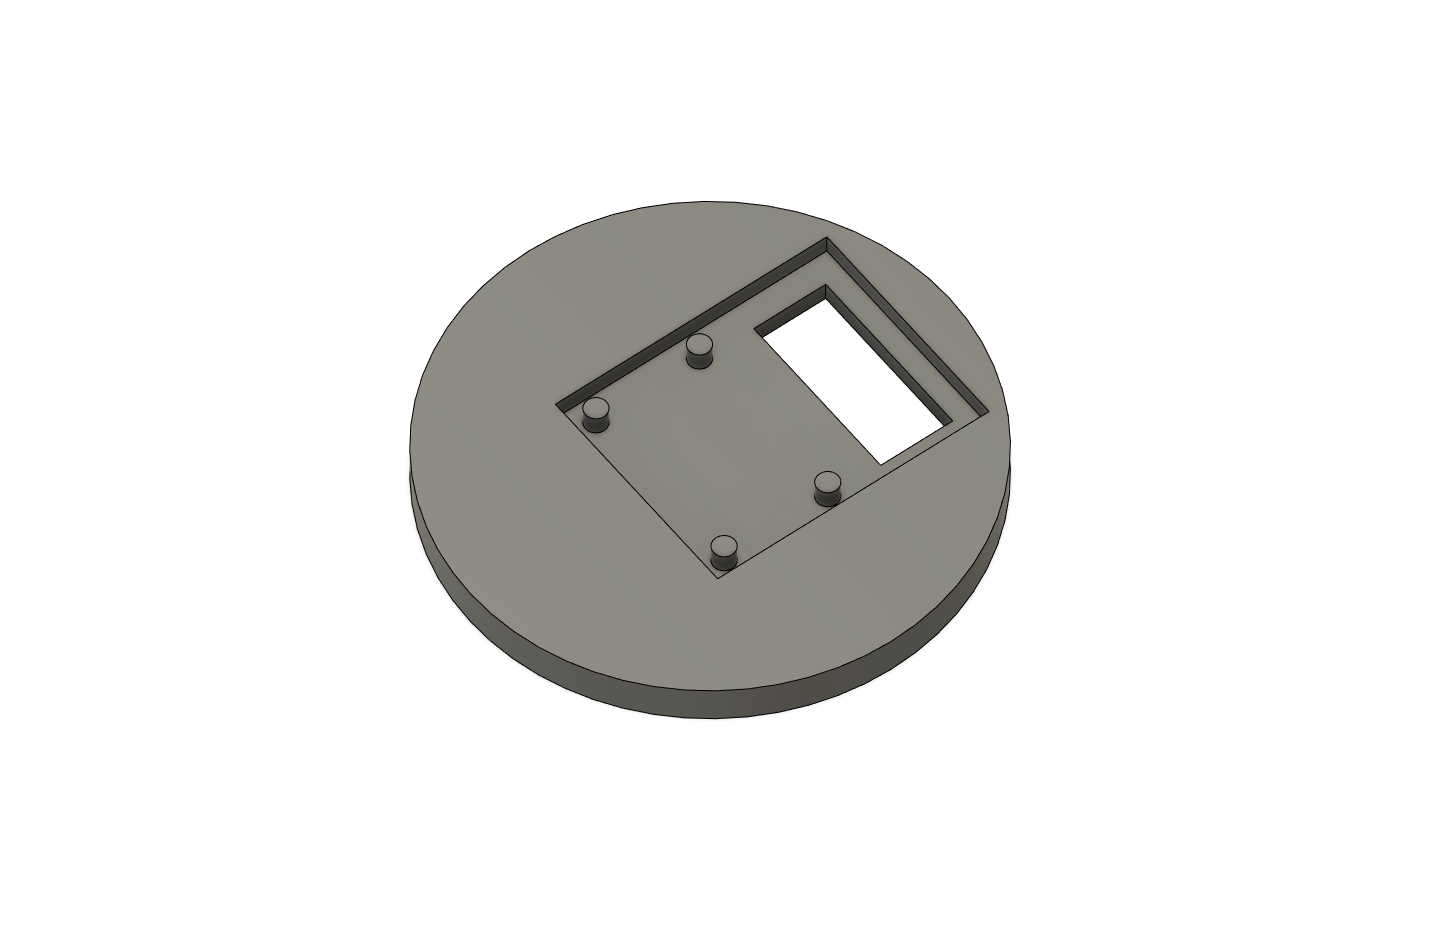
\includegraphics[width=0.5\linewidth]{assets/image.png}
    \caption{Bodenplatte um das Adapterplätchen richtig zu positionierten}
    
\end{figure}
In der Vertiefung für die Adapterplatte ist am äusseren Ende eine rechteckige Lücke ausgespart. Durch diese können die Anschlusskabel von der Adapterplatte zum Raspberry Pi Zero W 1.1 und zum Ground Leiter der Stromversorgung geführt werden. 

Der gesamten Windrichtungssensor ist 15 cm hoch und wird an der Sitzes des Bootes mit der Deckplatte verklebt.
\begin{figure}[H]
    \centering
    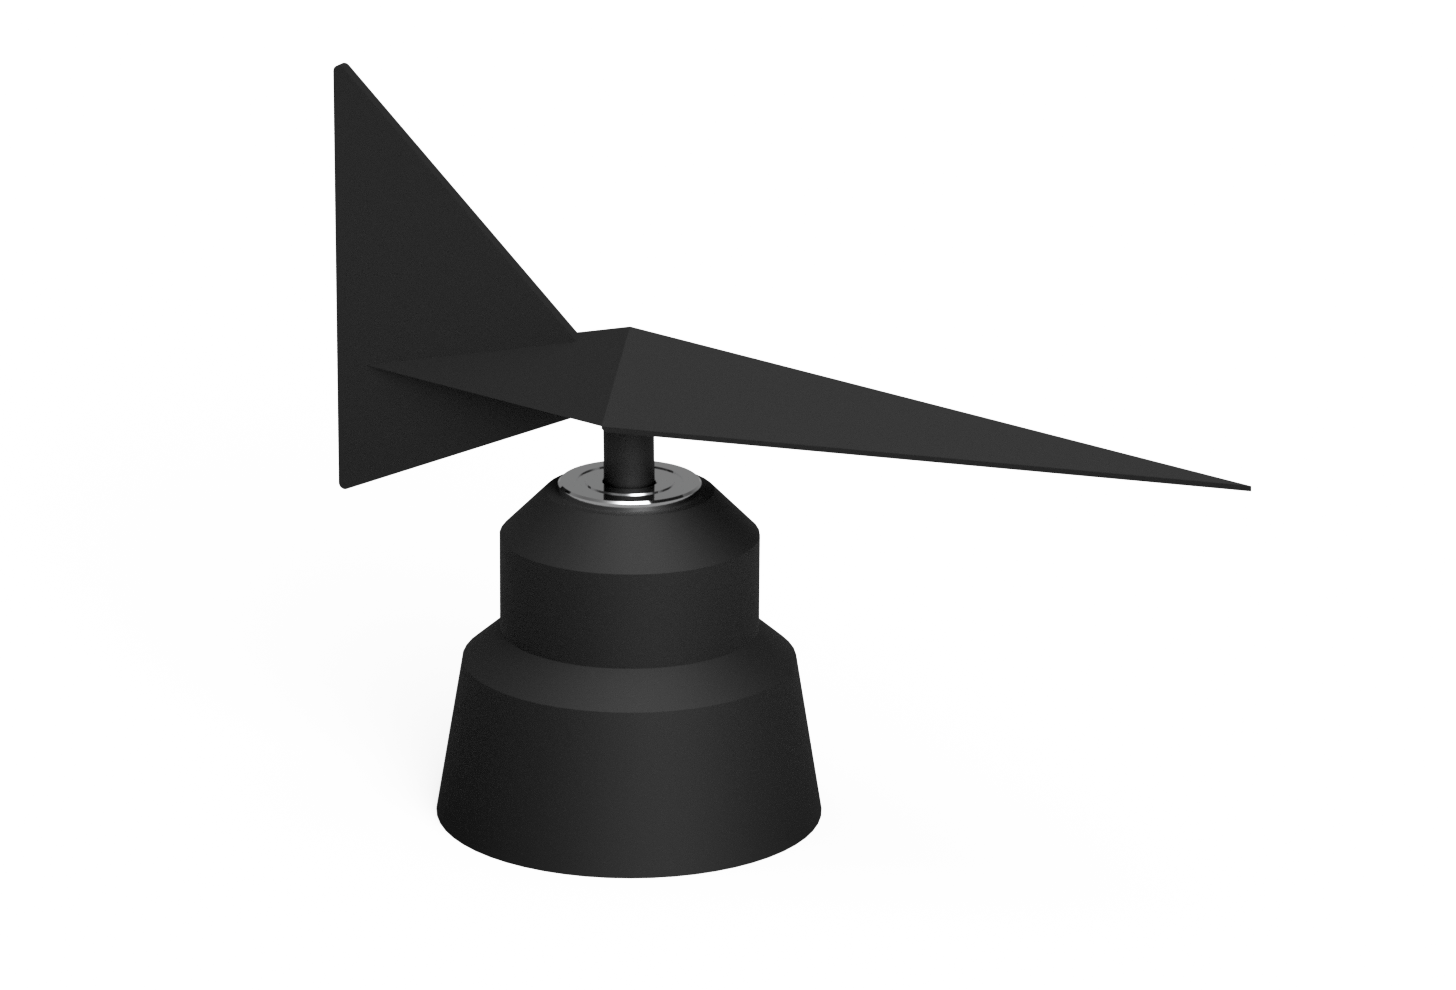
\includegraphics[width=0.75\linewidth]{assets/full_wind_sensor.png}
    \caption{Kompletter Windrichtungssensor}
    \label{fig:enter-label}
\end{figure}

\subsection{Aktuatoren}
Für die Bewegung des Ruders und des Sailflaps werden Aktuatoren verwendet. Aktuatoren (auch als Aktoren bezeichnet) sind das signalwandlerbezogene Gegenstück zu Sensoren. Sie setzen bei einem Bewegungsregelungsvorgang Signale durch mechanische Arbeit in Wirkungen um \cite{noauthor_aktor_2023}. Zur Bewegung von Ruder und Sailflaps werden elektrische lineare Aktuatoren benötigt. Ein elektrischer Linearantrieb ist ein Gerät, das die Drehbewegung eines Wechsel- oder Gleichstrommotors in eine lineare Bewegung umwandelt. Er kann sowohl Schub- als auch Zugbewegungen ausführen.

Für das vorliegende Projekt werden zwei L16-100-63-6 Serie R Aktuator der kanadischen Actuonix Motion Devices Inc. verwendet. Diese sind für den Einsatz in der Robotik und im Modellbau entwickelt worden und wasserdicht. Damit sind sie für den Einsatz auf Segelbooten prädestiniert.

Die Aktuatorrwelle aus Aluminium verfügt über einem Maximalhub von 100 mm. Die Maximalgeschindigkeit liegt ohne Last bei 20 mm/s. Damit sind sie nicht besonders schnell, verfügen mit 100N Stoss- und 46N Zugkraft aber über ausreichen Kraft zur Bewegung von Ruder und Sailflaps. Ihr Peak Power Point (der spezifische Geschwindigkeits- und Kraftpunkt, an dem die grösste Leistungsabgabe erfolgt) liegt bei 75N bei 10 mm/s. Das Getriebe der Aktuatoren weist eine Übersetzung von 63:1 auf.

\begin{figure}[H] 
    \centering
    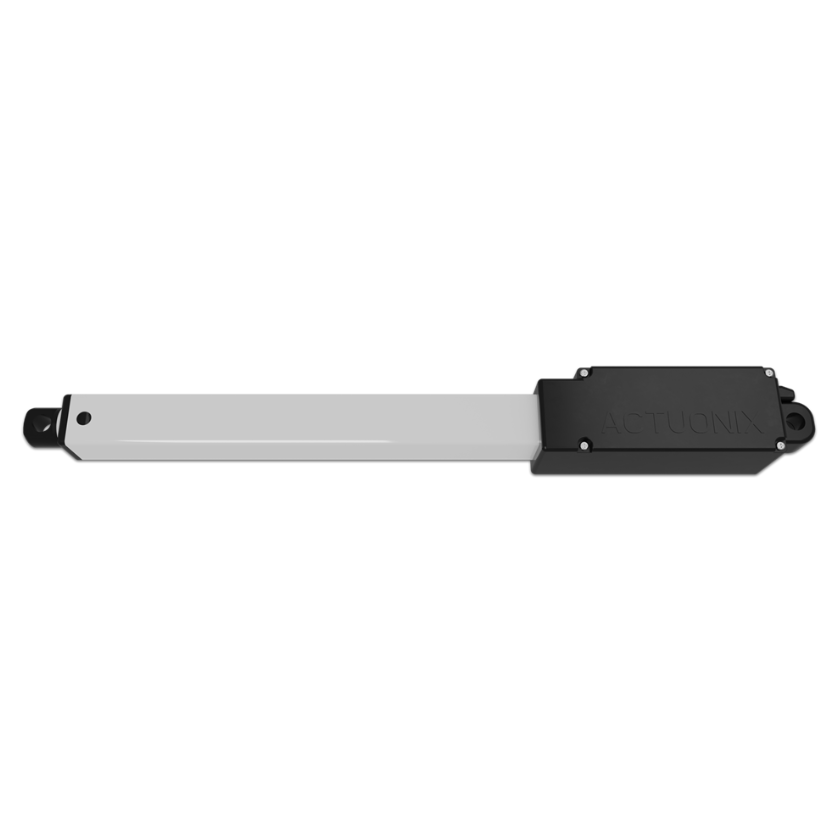
\includegraphics[width=0.75\linewidth]{actuonix.png}
    \caption{Actuonix Aktuator}
    \label{fig:actuator}
\end{figure}

Die Aktuatoren verfügen über kein digitales Positionsfedback, dass heisst, dass nicht abgefragt werden kann, an welcher Position sich das Ende der ausfahrbahren Welle befindet. Es können jedoch konkrete Distanzen angesteuert werden. 

Die Aktuatoren verfügen über kein digitales Positionsfedback, dass heisst, dass nicht abgefragt werden kann, an welcher Position sich das Ende der ausfahrbaren Welle befindet. Es können jedoch konkrete Distanzen angesteuert werden. 

Über eine einzige Datenleitung können kurze Impulse zwischen 1ms-2ms gesendet werden, wobei 1ms den Aktuator in die Startposition führt und der Aktuator bei 2ms voll ausgefahren wird. Um Einstellungen dazwischen zu erhalten, wird ein Wert zwischen 1ms und 2ms gesendet. 

Die Steuerleitung des Aktuators kann nicht direkt mit dem Raspberry Pi Zero W 1.1 verbunden werden, da dieser an seinen Pins nur 3,3 V Steuersignale ausgibt, der Aktuator aber ein 5 V Steuersignal erwartet. Aus diesem Grund muss zwischen den beiden Aktuatoren und dem Raspberry Pi Zero W 1.1 ein einfacher Pegelumsetzer (lever shifter) geschaltet werden. Es wird das Modell  BOB-12009 des US-amerikanischen Herstellers SparkFun Electronics verwendet.

\begin{figure} [H]
    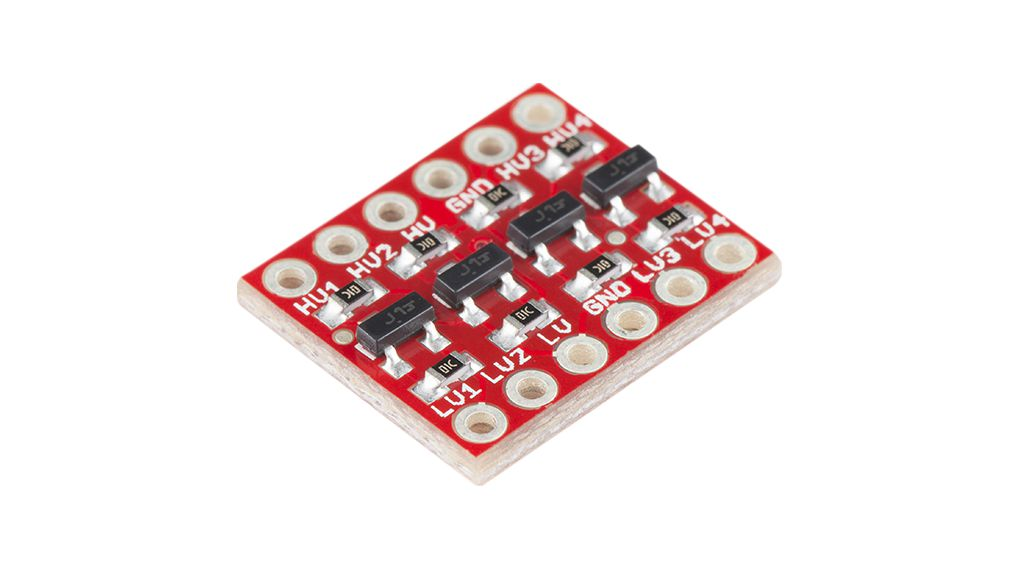
\includegraphics[width=1\linewidth]{assets/Sparkfun-BOB-12009-30145425-01.jpg}
    \caption{Pegelumsetzer}
    \label{fig:enter-label}
\end{figure}
Zur Ansteuerung wird die am ersten Pin des Ruderaktuators befestigte weisse Kabelize mit einem Verlängerungskabel mit dem Pin 1 (LV1) der linken Pinleiste des Pegelumsetzers verbunden und der Pin 1 (HV1) der rechten Pinleiste mit dem Pin 15 des Raspberry Pi Zero W 1.1 verbunden. Die am ersten Pin  des Sailflapaktuatoirs befestigte weisse Kabelizes wird mit einem Verlängerungskabel zunächst in den Mast und dann durch den Schleifring geführt und mit dem Pin 2 (LV2) der linken Pinleiste des Pegelumsetzers verbunden. Der Pin 2 (HV2) der rechten Pinleiste wird dann mit dem Pin BCM 4 des Raspberry Pi Zero W 1.1 verbunden.

\section{Schleifring (Slip Ring)}
Der Aktuator zur Bewegung der Sailflaps muss einerseits über den Pegelumsetzer mit dem Raspberry Pi Zero W 1.1 und andererseits mit der Stromversorgung verkabelt werden. Da das Segel frei rotiert und sich um die eigene Achse drehen kann, besteht die Gefahr, dass die Verbindungskabel um den Mast gewickelt werden und reissen.

Dieser Gefahr kann mit dem Einsatz eines sogenannten Schleifrings begegnet werden.  Ein Schliefring ist ein elektromechanisches Bauteil, das eine elektrische Leistungs- oder Signalübertragung zwischen gegeneinander rotierenden Bauteilen ermöglicht. Er besteht aus einem stromleitenden Ring und Bürsten, die in Kontakt mit diesem Ring stehen. Die Bürsten bestehen aus einem leitfähigen Material und sind mit der stationären Struktur des Systems verbunden. 


Der Schleifring wird am Fuss des Segelmastes montiert und mit dem Schiffskörper verschraubt. Durch den hohlen Mast werden dann die drei Leistungen hinauf zum Segel gezogen und durch ein in den Mast gebohrtes Loch zum Aktuator geführt und mit diesem verbunden.   

\section{Energieversorgung}

Rechner, Sensoren und Aktuatoren werden mit elektrischer Energie betrieben. Weil das Segelboot autonom funktionieren soll, muss diese auf dem Schiff selbst gewonnen werden. Infrage kommen dabei grundsätzlich drei Energiequellen, nämlich Wasserenergie, Windenergie und Sonnenenergie.

\subsection{Wasserturbine}
Da sich das Boot im Wasser bewegt, könnte eine kleine Wasserturbine am Bootskörper befestigt und die Strömung zu deren Antrieb genutzt werden. Da sich das Boot relativ zum Wasser bewegt, gelten die gleichen Prinzipien wie bei Generierung elektrischer Energie durch Wasserkraft in Fliessgewässern.

Diese Methode hat jedoch gewichtige Nachteile. Segelboote erreichen, abgesehen von speziellen Konstruktionen wie sog. Foilingboote, bei denen der Bootskörper bei Fahrt vollständig aus dem Wasser gehoben wird, nur bescheidene Geschwindigkeiten. Da die Leistung einer Turbine in einer Flüssigkeit bei gleicher Fläche kubisch zur Strömungsgeschwindigkeit ansteigt, erlaubt diese Methode selbst bei idealen Segelbedingungen nur eine geringe Energieausbeute. Zudem würde das Segelboot durch die Turbine empfindlich abgebremst. 

\subsection{Windturbine}
Auch die Generierung von elektrischer Energie mithilfe einer Windturbine unter Nutzung der Windkraft ist nicht praktikabel. Um die Windenergie in Bewegungsenergie umzusetzen, aus der dann elektrische Energie generiert werden kann, muss ein Windrad in den Wind gedreht werden. Ein Segelboot kann keinen Kurs gegen den Wind segeln. Der Kurs vor dem Wind (also ein Kurs, bei dem der Wind von hinten auf das Boot trifft) ist zwar möglich, aber wenig effizient. Ein Windrad könnte folglich nicht fix mit dem Boot verbunden werden, sondern müsste drehbar ausgelegt werden, damit es unabhängig vom Kurs des Bootes in den Wind gedreht werden kann. Es müsste so platziert werden, dass nicht nur eine Berührung des Segels, sondern auch eine Berührung der Wasseroberfläche bei einer Kränkung (Schieflage) des Bootes ausgeschlossen ist. Damit müsste es am äussersten Bug, am äussersten Heck oder auf dem Mast platziert werden. Alle Positionen verbieten sich, da damit die Balance des Bootes akut gefährdet wäre. 

Schliesslich würde eine Positionierung am Bug oder Heck je nach vorherrschendem Wind, zu einer vollen oder teilweisen Abschattung des Windrades durch das Segel oder des Segels durch das Windrad führen. Eine Positionierung auf dem Mast würde selbst im Fall eines Vertikalwindrades zu Verwirbelungen führen, welche die Segeleigenschaften des Bootes negativ beeinträchtigen würden.

Einfluss auf den Kurs, da das Boot nicht verankert ist. Damit geht Energie verloren, da das Boot „weggeschoben“ wird, statt die Windenergie in nutzbare Drehung umzusetzen.

\subsection{Photovoltaik}
Für die Nutzung der Sonnenenergie auf dem autonomen Segelboot kommt nur die Methode der Fotovoltaik infrage. Die für den Betrieb von Wärme-Kraft-Maschinen erforderlichen Temperaturen lassen sich auf einem beweglichen Boot mit Sonnenenergie nicht erreichen.

Die Energieerzeugung mit Fotovoltaikanlagen ist auf Segelbooten beliebt und verbreitet. Solche Anlagen haben keinen Einfluss auf die Segeleigenschaften des Bootes. Die Energieausbeute hängt aber stark vom Sonnenstand und dem vorherrschenden Wetter ab. Im Gegensatz zu stationären Anlagen lassen sich Fotovoltaikanlagen auf Booten nicht ideal auf die Sonne ausrichten und können je nach Kurs sogar vom Segel beschattet werden. Da während der Nachtstunden überhaupt keine Energie gewonnen werden kann, muss das Boot zur Überbrückung zwingend mit einem Energiespeicher ausgerüstet werden.

Das Solarpanel kann auf dem Deck oder am Festsegel befestigt werden. Die Befestigung auf dem Deck hat den Vorteil, dass die Verbindungsleitung zum Energiespeicher nicht durch den Schleifring geführt werden muss. Sodann ist die sichere Befestigung am flachen Deck einfacher als am gewölbten Festsegel. Schliesslich müssten bei einer Montage am Segel zwei Panels verwendet werden, damit beiden Seiten des Festsegels damit ausgerüstet werden können. Andernfalls bestünde die Gefahr, dass sich das Panel bei einem ungünstigen Kurs längere Zeit auf der Schattenseite des Festsegels befindet.  

Der Selbstbau eines Panels wird nach einer längeren Erkundungsphase verworfen, da komplette, für den mobilen Einsatz entwickelte Panels kostengünstiger sind.   

Es wird das portable und faltbare PiJuice Solar Panel - 22 Watt der britischen Pi Supply (Nebra Ltd verwendet. Es ist gegen Spritzwasser geschützt (IP4X-Kennzeichnung), misst im entfalteten Zustand 83x23 cm und wiegt 520 g. Die vier einzelnen Panele sind von einer Textilhülle umfasst, die vier Befestigungsösen aufweist. Mit diesen wird das Panel vor dem Mast auf der flachen Deckplatte des Segelboots befestigt.

Die maximale regulierte Ausgangsleistung beträgt 20 W bei 5 V. Es verfügt über zwei 5 V/ 2.4 A USB Ausgänge, wobei die maximale Ausgangsleistung pro USB Buchse auf 12 W beschränkt ist. Die zwei USB Buchsen können simultan benutzt werden.
\begin{figure}[H]
\centering
    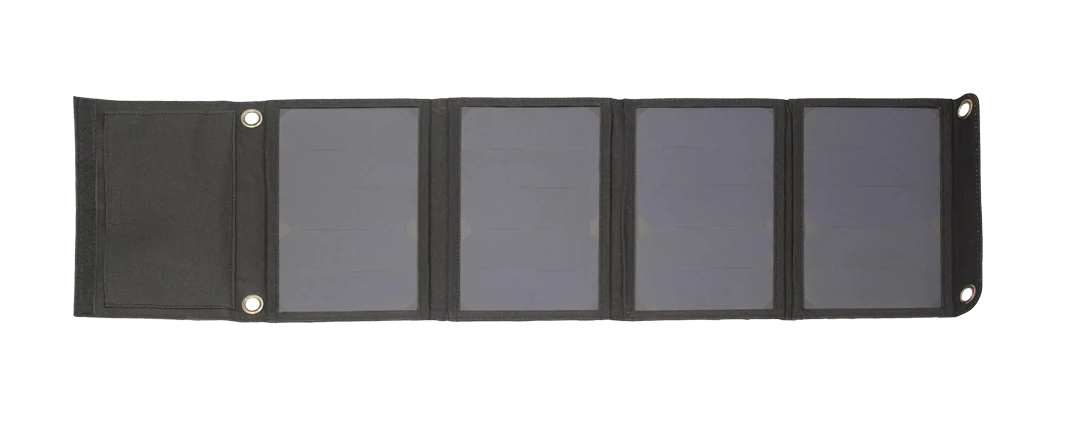
\includegraphics[width=1\linewidth]{assets/Pi juce.png}
    \caption{Pi Juce Solarpanel}
    \label{fig:enter-label}
\end{figure}
\subsection{Enegiespeicher (Akku)}
Während der Nachtstunden kann mit dem Solarpaneel keine Energie gewonnen werden kann und bei Nebel ist die Energieausbeute sehr gering. Daher muss das Boot zur Überbrückung dieser Phasen mit einem Energiespeicher ausgerüstet werden, damit seine Autonomie sichergestellt ist.

Es wurde vorgesehen, dass die Energiereserve einen Betrieb während drei Tagen (72 h) erlauben soll. Der genaue Energieverbrauch des Rechners, der Sensoren und vor allem der Aktuatoren hängt stark davon ab, wie oft Steuereingriffe vorgenommen werden müssen und Messdatenerfassungen Neuberechnungen erfolgen. Es lässt sich daher nicht präzis berechnen, sondern nur abschätzen.

Der Schätzwert für den Gesamtenergieverbrauch pro Stunde beträgt 1.5 Watt (bei 5 Volt Gleichspannung). Das ergibt einen Energieverbrauch von 36 Wattstunden pro Tag (24 h). Zur Überbrückung der vorgesehenen drei Tagen ohne Energiezufuhr muss der Speicher daher über eine Kapazität von mindestens 108 Wattstunden verfügen. 

Eine völlige Erschöpfung des Energiespeichers kann diesen schädigen. Sie muss daher verhindert werden. Aber bereits ein Absinken der Ladung auf unter 20 Prozent verkürzt dessen Lebensdauer. Die Kapazität muss daher erhöht werden. Um über ausreichen Reserven zu verfügen, wird daher eine Kapazität von 185 Wattstunden vorgesehen.

Im Handel erhältliche sogenannte Powerbanks verfügen über eine Kapazität von bis zu 20'000 mAh, was eine Leistung von 100 Wh ergibt. Eine solche Powerbank genügt den gestellten Anforderungen damit nicht. Auch eine Kombination mehrerer Powerbanks scheidet aus, weil heute angebotene Geräte nicht auf die sogenannten Durchgangsladung (pass‐through charging) ausgelegt sind. Sie können also nicht geladen werden, während ein Verbraucher Energie bezieht.  

Deutlich grössere Powerstations, die insbesondere für den Campingeinsatz vorgesehen sind, verfügen über deutlich grössere Kapazitäten und sind duchgangsladungsfähig. Sie sind aber meist auf Verbraucher ausgelegt, die mit 220 V Wechselspannung betrieben werden, sind meist weit über 10 Kg schwer und kosten über 1000 Franken. Sie scheiden damit ebenfalls aus. 

Der Energiespeicher muss daher selbst entworfen und gebaut werden. Bei Selbstbauprojekten werden dafür häufig Li-Ion Zellen der Bauform 18650 verwendet.

Für den Energiespeicher sollen 20 günstige wiederaufladbare EVE ICR18650/ 26V Litium-Ionen Zellen der chinesischen EVE Energy CO., LTD verwendet werden. Die Zellen haben eine Kapazität von 2'550 mAh bei 3.7 V.
 \begin{figure}
     \centering
     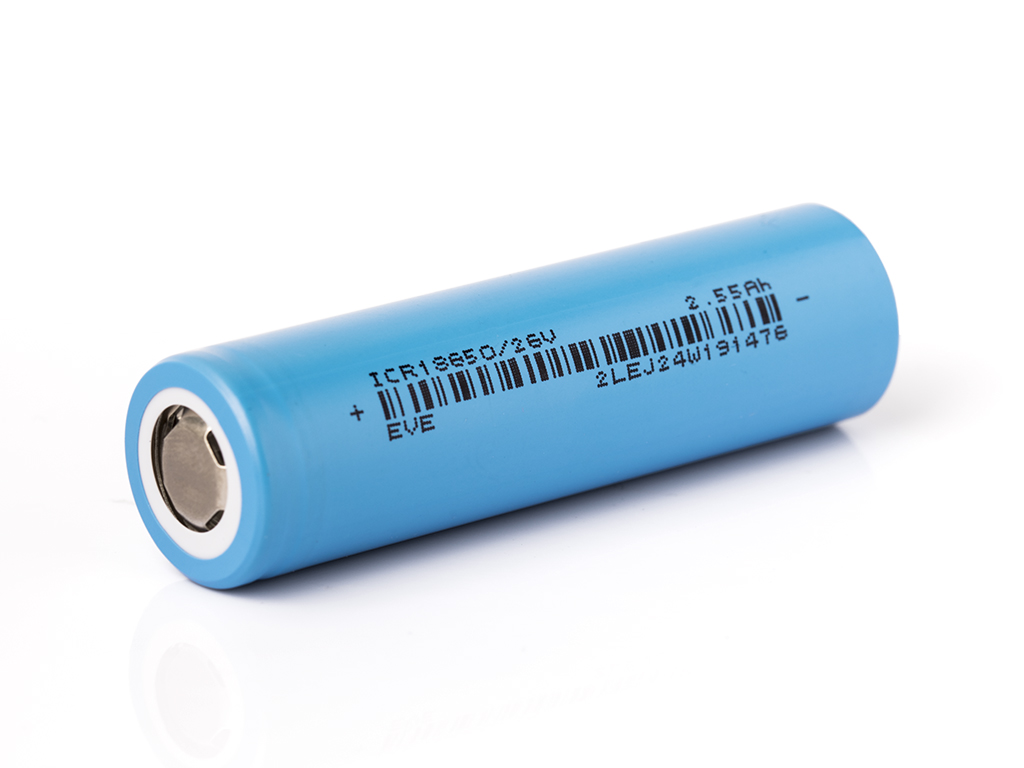
\includegraphics[width=0.5\linewidth]{assets/EVE-ICR18650-26V-3-6V-3-7V-2600mAh-7-5A-Li-Ionen-Akku.jpg}
     \caption{ EVE ICR18650/26V Litium-Ionen Zelle}
     \label{fig:enter-label}
 \end{figure} 
   
   
Der Energiespeicher (Akku) wird aus zwei identischen Teilen mit je 10 Zellen aufgebaut. Die Zellen werden innerhalb ihres Zellverbundes parallel geschaltet. Damit bleibt die Spannung der Zellen unverändert, aber die Kapazität des Zellenverbunds erhöht sich. Die beiden Zellverbände werden seriell geschaltet, womit sich eine Spannung des Akkus von 7.4 V und eine Kapazität von 25000 mAh ergibt.

Die einzelnen Zellen jedes Zellverbundes werden untereinander mit einem Nickelband verbunden, das mit einem Punktschweissgerät direkt auf den Zellen geschweisst wird. Das Punktscheissgerät muss speziell für dies Projekt angeschafft werden, da ein solches Spezialwerkzeug nicht zur Standardausrüstung einer Heimwerkerwerkstatt gehört. Es wäre an sich möglich, die Nikkelbänder mit den Zellen zu verlöten. Dabei besteht aber die ernste Gefahr, dass die Zellen mit dem Lötkolben zu lange und zu stark erhitzt werden. Sie können dabei nicht nur unrettbar beschädigen werden, sondern sich auch entzünden. Aus Sicherheitsgründen wird daher von den definierten Anforderungen abgewichen.
 \begin{figure}
 \centering
    \includegraphics[width=1\linewidth]{assets/akku_transparent.png}
    \caption{Selbstgebauter Akku}
    \label{fig:enter-label}
\end{figure}
\subsection{Ladeeletronik und Spannungswandelung}

Da Lithiumzellen bei einer Überladung oder bei einer Tiefentladung beschädigt oder im schlimmsten Fall in Flammen aufgehen können, wird ein \ac{bms} (Battery Managment System) Modul verwendet. Dieses wird mit dem Plus und Minus Pol des Akkus verbunden. Zudem gibt es eine PM-Verbindung, nach dem ersten Teil der seriellen Hälfte.


\begin{figure}
    \centering
    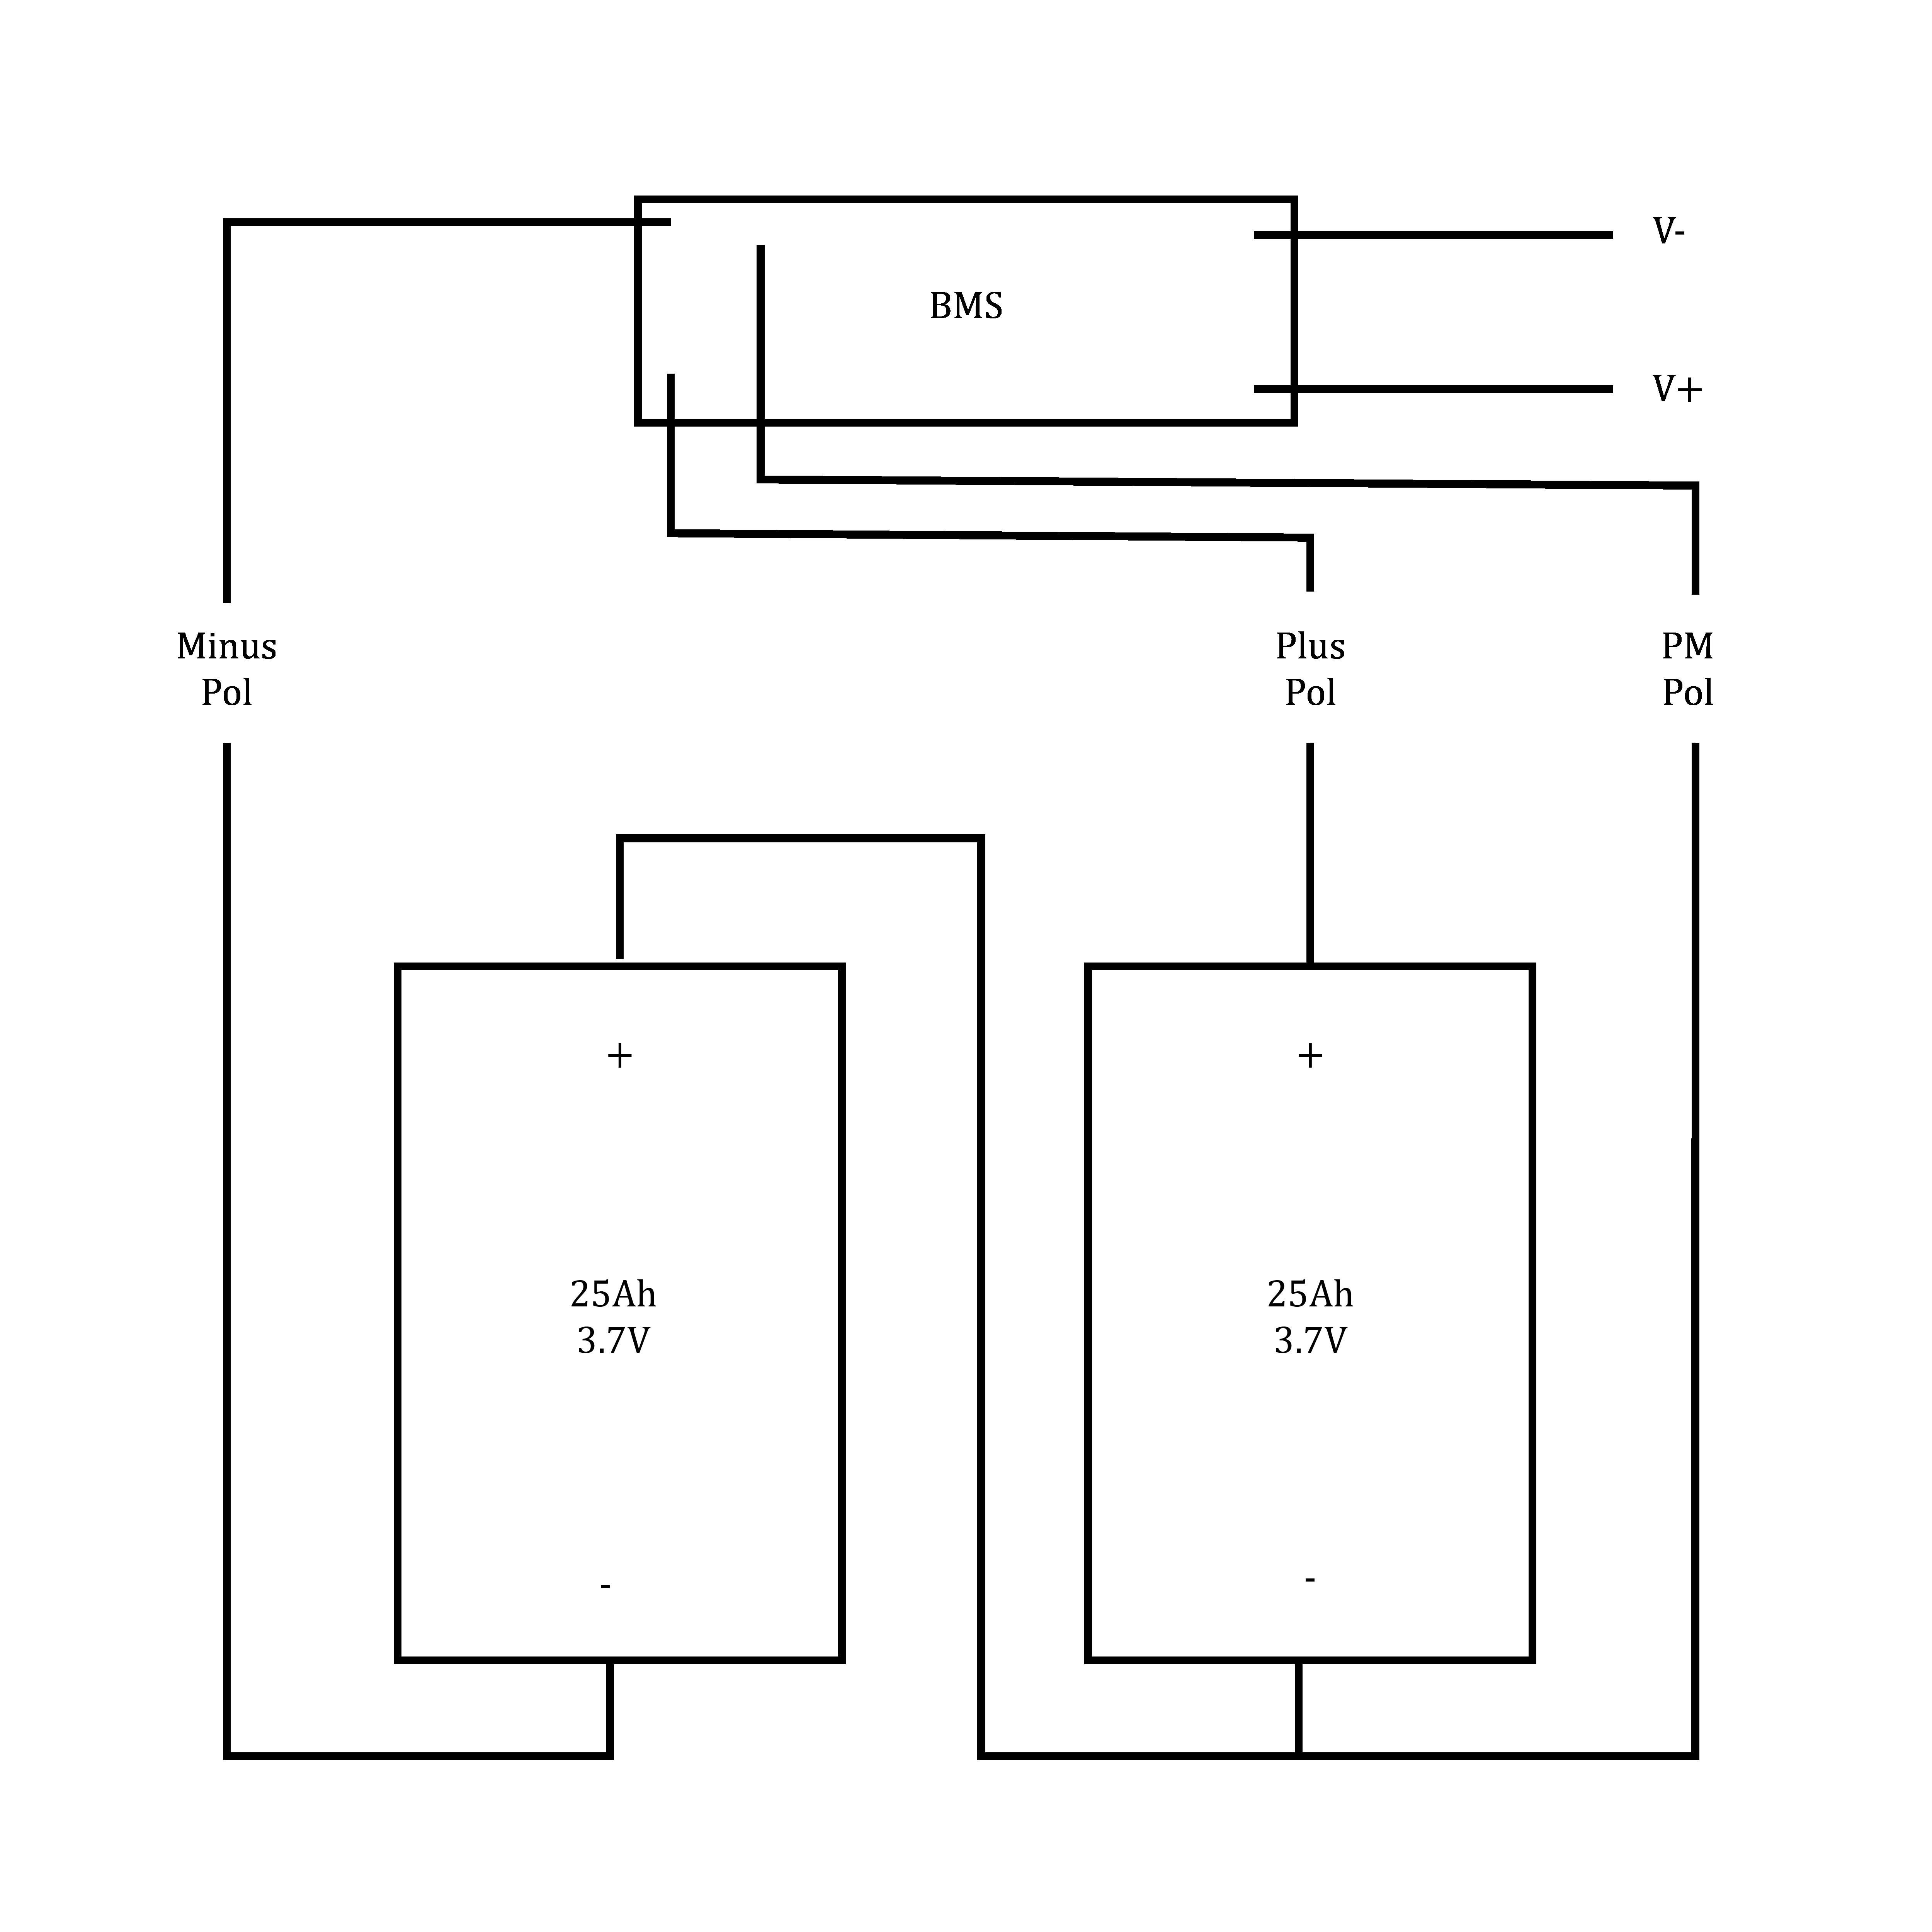
\includegraphics[width=0.5\linewidth]{assets/bms_circuit_image.png}
    \caption{Ladeelektronik-Schaltkreis}
    \label{fig:enter-label}
\end{figure}
